\chapter{Experiment Design and Results}
\label{ch:experiment}

% TODO: Scrivi intro
\paragraph{}

 
\section{Neural Network Architecture and Training Algorithm}
\label{sec:nn}
\paragraph{} One issue with GAN models is that the loss function is not always correlated with the generated sample quality, added to the problem of evaluating the sample quality. Although we tried some different \glspl{gan} implementations and techniques, our principal selection criterion has been the effectiveness on our particular dataset of the proposed solution in solving this stability problems.

\subsection{Network Architecture}
\label{sec:networkarch}

\subsubsection{Chosen Architecture} 
\paragraph{} Among the various \glspl{gan} implementations that are proposed in the literature, we selected the Wasserstein GAN with Gradient Penalty \cite{wgangp} (WGAN-GP) described in section~\ref{sec:wgangp} as it showed better training stability with the DCGAN layer configuration and at least comparable sample quality as opposed to the other models.


\subsubsection{Loss Formulation}
\paragraph{} We implement the Critic and Generator losses as in the \citetitle{wgangp} official implementation \cite{wgangp-imple}, which combines formulas \ref{eq:wganloss} and \ref{eq:gp}. Referencing to the notation introduced in \ref{sec:modelstructure} the losses are defined as follow:

\begin{equation}
\label{eq:loss}
 \begin{split}
L_{Critic}^{(i)} \gets & \underbrace{\operatorname{E}(Logits(X_{Gen})) - \operatorname{E}(Logits(X_{True}))}_{\text{WGAN Loss}} + \underbrace {\lambda G_p}_{\text{Gradient Penalty}} \\
%\tag{WGAN-GP Generator Loss}
L_{Gen}^{(i)} \gets & -Logits(X_{Gen}) 
\end{split}
\end{equation}

where $X_{True}$ and $X_{Gen}$ are batches of levels sampled respectively from the dataset and the generator network, $\lambda = 10$ and $ \epsilon \sim U[0,1] $ (for the gradient penalty), in our experiments.

\paragraph{} We can now give an intuitive interpretation of the loss we used: The critic network is trained, by minimizing \ref{eq:loss}, to assign a "score" to real and generated samples. This is one of the reasons that motivate the change in name from "discriminator" to "critic"~\footnote{ Comments about the Wasserstein GAN paper from the authors of WGAN and GAN papers, among the others: \url{https://www.reddit.com/r/MachineLearning/comments/5qxoaz/r_170107875_wasserstein_gan/}}, since the network outputs are in this case not probabilities but unbound values.

\subsubsection{Training Algorithm and Hyper-Parameters}
For implementing the training algorithm we followed the algorithm suggested by \cite[alg.~1. p.~4]{wgangp}, which uses \textit{Adam}\cite{adam} as the optimizer for both the networks and optimizes $n_{critic} = 5$ times the critic network for each generator update. \\*
In addition to this implementation, we also imposed an input rotation of 90° for each sample at each epoch, such that each 4 epochs the network had in input all the possible orientation of a level. This allows us to exploit the rotation invariance in the representation of a level, since its playability is not affected by its orientation in the space it is represented. Table \ref{tab:training} shows in detail the frequency of each computation operation relative to each critic step, with reference to our TensorFlow implementation at \cite{gitrepo}. Due to implementation constraints, we calculate the Metrics out of the TensorBoard computation graph, so they appear as inputs since they have to be visualized with the other values. Reference Sample refers to the computation of a sample that is generated by the same $Y$ and $Z$ vectors, sampled at the beginning of the training phase. This helps in visualizing how the network weights optimization visually impact on the generation of one sample. \\*
 The  hyperparameters we used in our experiments are $\alpha=0.0002, \beta_1=0, \beta_2, \lambda=10$.
 


\begin{table}[h!]
	\centering
	\begin{tabularx}{\textwidth}{| c | X | X | X | X | c | X | }
		\hline
		Run Name & \multicolumn{3}{X|}{Inputs} & Outputs & Frequency & Evaluated operators \\ \cline{2-4}
		  & Critic Input ($X_{True}$) & Scalar Features $(Y)$ & Generator noise (Z) &   &   &   \\
		\hline
		Train G & - & $Y_{Train}$ & $U[0,1]$ & $L_{Gen}$ & $5$ & $G_{optim}$, $summary_D$ \\ \hline
		Train D & $X_{Train}$ & $Y_{Train}$ & $U[0,1]$ & $L_{Critic}$ & $1$ & $G_{optim}$, $summary_D$\\ \hline
		Validation & $X_{Val}$ & $Y_{Val}$ & $U[0,1]$ &  $L_{Gen, Val}$, $L_{Critic, Val}$, $X_{Gen}$ & $100$ & $G_{optim}$, $summary_D$ \\ \hline
		Metrics & \multicolumn{3}{X|}{$Metrics(X_{Val}, X_{Gen})$} &  - & $100$ & $G_{optim}$, $summary_D$ \\ \hline
		Reference Sample & $-$ & $Y_{Ref}$ & $Z_{Ref}$ &  $X_{Ref}$ & $100$ & $G_{optim}$, $summary_D$ \\ \hline
		Network Checkpoint & $-$ & $-$ & $-$  & checkpoint & $100$ & $save()$ \\ \hline
	\end{tabularx}
	\caption{Training Algorithm Operations}
	\label{tab:training}
\end{table}








\subsubsection{Artefacts Reduction}
\paragraph{} One of the problem that often affects GAN is the presence of artefacts or regular patterns in the generated samples. This problem can be less noticeable when the network is generating images of real objects such in the majority of used dataset, but it's an important issue in our setting in which a change in a pixel can have noticeable impact on the resulting level and its associated metrics. This problem is well explained in \cite{artifacts} and it's due to how the transposed convolution is applied in case the kernel size is not divisible by the stride. In this case the convolution leads to an un-even overlap of outputs in the high-resolution image, generating the artefacts. Among the proposed solutions to overcome this issue we chose to simply use a kernel size of 4 and a stride of 2, which showed to reduce the problem in our case without impacting on performances or layer architecture. 



\section{Input selection, Metrics and Sample Method}
\label{sec:input_metrics_sample}
\subsection{Input data}
\label{sec:InputSelection}
\paragraph{} For our experiments we filtered the DoomDataset by taking only the samples up to 128x128 in size and which had exactly 1 "floor". This led to a dataset of about 1000 samples, which are then augmented by rotation during the training process. This is motivated from the fact that even if the level orientation does not affect playability, using levels with more floors could lead the network to learn a correlation between floors (and how to arrange them inside the map) which could potentially be misleading or be just enforced by the sample size or the way the editor arranged them on the level coordinate space. Moreover, using only one-floor levels helped in reducing smaller artefacts that appeared as very small floors in resulting output.

\subsection{Sample Evaluation metrics}
\label{sec:evaluation}
\paragraph{} The problem of evaluating the quality of the samples generated from a neural network remains an open area of research \cite{improved_gan}. The architectures that we considered are primarily trained on datasets consisting of images representing real objects, such as faces or bedrooms. For dealing with this problem, \citeauthor{improved_gan} propose both a process in which human annotators are asked to assess the perceived quality of the samples \cite[p.~4]{improved_gan} and the usage of the Inception Model \cite{inception} Score for assessing the perceived quality of the samples. Although many authors had success in assessing sample quality using the Inception Score, this method showed to perform poorly on our dataset. The most probable reason is that our dataset is very different from the ImageNet dataset upon which is trained the Inception Network. \\* Since tuning the Inception network to work with our dataset or applying other proposed solutions based on similarly complex models wouldn't have been possible given our computational constraints, we decided to design some heuristics that could correlate with sample quality at least with our dataset. These sample evaluation metrics give an additional measure for assessing the generated sample quality during the training process, while the final model performance is assessed by confronting the true and generated input distributions (Section \ref{sec:modelevaluation}).

\paragraph{} Instead of asking a neural network to evaluate the generated samples, our process compares two samples that have been generated by the network using the same conditioning vector. Since in principle, given a vector of scalar features $Y$, the network could generate samples which are topologically and visually very different, any metric that used quantities that are strictly related to the level topology rather than a perceived concept of "quality" couldn't lead to reasonable results. In designing these metrics we inspired to the paper \citetitle{slam}. In their work, \citeauthor{slam} propose their solution to the problem of evaluating the maps generated by a SLAM algorithm running on a mobile agent. Their approach consist in defining three metrics that capture different aspects of the analysed maps, which features some similarities with the \glspl{featuremap} we use, and considering the entire set of metrics as an approximation of the human perceived quality of a map. 
\\* Following a similar approach, we defined the following metrics for estimating the perceived quality of a sample generated by our network. These metrics are not meant to be a general solution to the problem of evaluating samples of a \gls{gan} nor to improve the work of \citeauthor{slam_metrics}, but only to be used as a quantitative tool for assessing the samples in our particular case.

\subsubsection{Entropy Mean Absolute Error}
This metric is defined as the Mean Absolute error between the entropy of two images in their colour space. In particular, since as described in chapter~\ref{sec:DatasetOrganization} we are representing maps as grey-scale images whose colour ranges between 0 and 255, we calculate the pixel distribution over each possible colour value $c$ of an image $x$, $P_{c}(x)$, then we calculate the entropy as:
\begin{equation}
	S(x) = - \sum_{c=0}^{255}{ P_{c}(x) * \log{P_{c}(x)} }
\end{equation}

then, the metric over a batch of true images $X_{true}$ and a batch of generated images $X_{gen}$, both consisting of $N$ samples, is calculated as:

\begin{equation}
Entropy_{mae}(X_{true}, X_{gen}) = \frac{1}{N}\sum_{i=0}^{N-1} | S(X_{gen}(i)) - S(X_{true}(i)) |
\end{equation}

This metric is related to how different the entropy of a generated image is from the corresponding real image, which can also be interpreted as the difference in the quantity of information expressed by the two samples. In general, large values of this metric indicates that the generated sample is very noisy or the topology of the two levels are greatly different, while small values indicates that the entropy of the two images are on a comparable level. 

\subsubsection{Mean Structural Similarity Index}
This metric is defined as the Structural Similarity (SSIM) Index \cite{ssim} between two images.  This measure is the result of a framework that consider several aspects of an image, such as the luminance, the contrast and the structure, rather than basing only on a statistic. Moreover, the structural similarity technique is applied locally over the image, for reflecting the fact that pixels are more dependant on other spatially close pixels than far ones. \\*
For calculating this metric we use the implementation provided by the Scikit-Image Python library, which we leave the formulation to the paper \cite[p.~604]{ssim}, and compute the mean of the SSIM index over the images belonging to the true and generated batches. Regarding the interpretation of the metrics, values closer to 1 indicate the fact that true and generated samples are often structurally similar: in other words, the network produces samples in which the local structure of the pixels are comparable.

\subsubsection{Mean Encoding Error}
We define as "Encoding Error" a measure of how far the pixels colour of a generated image are from their closest meaningful value. Specifically, as we introduced the encoding values for each feature map in chapter~\ref{sec:DatasetOrganization} the reader might have noticed that not all values correspond an actual representation. For example, the \gls{floormap} encodes the pavement as 255 and the empty space as 0, leaving values from 1 to 254 without a real meaning. Since as highlighted in section \ref{sec:usecases} the network only reads and outputs floating point numbers between 0 and 1, this is not actually a problem of choosing an encoding space for the images, rather it is intrinsic to the network definition. Due to the generation process involving noise and non-integer parameters, the network will often output pixel colours that are in-between the possible values the input images can take, even though this behaviour decreases as the training proceeds. \\*
The definition of this function, for a generic pixel colour value $x$ which assumes meaningful values every $i$ colour values, corresponds to a periodic triangular function having base $i$ which assumes the maximum value of $1$ wherever x is halfway a meaningful value and another. More formally:

	\begin{equation}
	Enc_{I}(x) \equiv \sum_{k \in Z} \Lambda (\frac{2(x-kI)-I}{I})
	\end{equation}
	

where $ \Lambda(x) $ is the unit-base triangular function such that $ \Lambda(0) = 1 $. \\*
The metric is then calculated as 

\begin{equation}
MEE(X_{gen}) = \frac{1}{N}\sum_{i=0}^{N-1} \frac{1}{|P|} \sum_{p\in P} Enc_I(p)
\end{equation}

where $p\in P$ is the colour of each pixel of the image, $|P|$ is the total number of pixels in an image and $N$ is the batch size of $X$. In particular, I is 255 for the \gls{floormap} and \gls{wallmap} while is 1 for the other maps.  \\*
Since, by construction, $MEE(X_{true}) = 0$ up to conversion errors or artefacts, this metric is only calculated for the generated samples and it is correlated with the ability of the network to represent precisely the data encoding.

\subsubsection{Mean Corner Error}
\paragraph{} This error is based on the idea introduced with the corner count metric introduced by \cite{slam}. We define our implementation of the Corner Error of two images as:
\begin{equation}
	C_{err}(n_{x}, n_{y}) = \sqrt{\frac{(n_{x} - n_{y})^2}{n_{x}n_{y}}}
\end{equation}
where $n_{x}$ and $n_{y}$ are respectively the corner count of two binary images, extracted using the Harris corner detector \cite{harrisdetector}.
This formula may seem arbitrary, but it demonstrated to scale well on our dataset, since the corner count is actually limited by the size of our samples. The final metric is computed, as the other cases, averaging the corner error over the images in the batch:

\begin{equation}
MCE(X_{true}, X_{gen}) = \frac{1}{N} \sum_{i=0}^{N-1} C_{err}(n_{true,i}, n_{gen,i})
\end{equation}
Again, for simplicity, we indicated as $ n_{true,i} $ and $ n_{gen,i} $ the corner count given by \\ $ n_{i} = count(peak(harris(X_{i}))) $, with obvious meaning of the function names.
This metric is proportional to the average distance that the true and generated samples have, giving a quantitative measure of relative map complexity. It is worth nothing that it's not always the case, since generation artefacts may dramatically increase this value, producing a great number of corners. For this reason, this quantity reflects both the relative average complexity between batches of images and the presence of noise or artefacts in the generated samples.

\subsection{Model Evaluation}
\label{sec:modelevaluation}
\paragraph{} In order to evaluate each model performance in a systematic way we designed an experiment for comparing the distribution of true data and the one generated from the neural network, according to the features that is possible to calculate from the output images. In particular we set up two evaluation experiments: The first generates a map for each feature vector taken from the dataset and compares the distributions of the real and generated datasets, for both input features and non-input features.
The second experiment selects a subset of different maps and considers the distribution of 1000 maps that are generated using the given input feature, for each map.

\paragraph{} 
%TODO: continue this, explain more what the experiments mean



\section{Trained Models}
\label{sec:experiments}
\paragraph{} We ran different input and layer settings for finding if one performed better than the others. In particular we kept fixed the WGAN-GP architecture, learning hyperparameters, the kernel size and the stride, while we varied the input features and the number of layers. \ref{tab:experiments} shows the details of each run.

\paragraph{} %TODO: Parla della selezione delle feature

\begin{table}[h!]
	\begin{tabularx}{\textwidth}{| c | c | X | X | X | X |}
		\hline
		\textbf{Run Name} & \textbf{Iterations} & \textbf{Features} & \textbf{Maps} & \textbf{D Layers (filters)} & \textbf{G Layers (filters)} \\
		\hline
		26k & 26000 & 
		\begin{itemize}
			\raggedright
			\small
			\item[] level equivalent diameter
			\item[] level major axis length
			\item[] level minor axis length
			\item[] level solidity
			\item[] nodes
			\item[] distmap-skew
			\item[] distmap-kurt
		\end{itemize}
		 & 
		 	\begin{itemize}
		 	\raggedright
		 	\small
		 	\item[] floormap
		 	\item[] heightmap
		 	\item[] wallmap
		 	\item[] thingsmap
		 \end{itemize}
		 & 4 (1024, 512, 256, 128) & 4 (128, 256, 512, 1024)\\
		
		\hline
		
		12k & 12000 & 
		\begin{itemize}
			\raggedright
			\small
			\item[] level equivalent diameter
			\item[] level major axis length
			\item[] level minor axis length
			\item[] level solidity
			\item[] nodes
			\item[] distmap-skew
			\item[] distmap-kurt
		\end{itemize}
		& 
		\begin{itemize}
			\raggedright
			\small
			\item[] floormap
			\item[] heightmap
			\item[] wallmap
			\item[] thingsmap
		\end{itemize}
		& 4 (1024, 512, 256, 128) & 4 (128, 256, 512, 1024)\\
		
		\hline
		
		unconditional & 15000 & 
		No features
		& 
		\begin{itemize}
			\raggedright
			\small
			\item[] floormap
			\item[] heightmap
			\item[] wallmap
			\item[] thingsmap
		\end{itemize}
		& 4 (1024, 512, 256, 128) & 4 (128, 256, 512, 1024)\\
		
		\hline
		
		deeper & 11000 & 
		\begin{itemize}
			\raggedright
			\small
			\item[] level equivalent diameter
			\item[] level major axis length
			\item[] level minor axis length
			\item[] level solidity
			\item[] nodes
		\end{itemize}
		& 
		\begin{itemize}
			\raggedright
			\small
			\item[] floormap
			\item[] wallmap
			\item[] thingsmap
		\end{itemize}
		& 8 (1024, 1024, 512, 512, 256,  256, 128, 128) & 8 (128, 128, 256, 256, 512, 512, 1024, 1024)\\
		\hline
		
	\end{tabularx}
	\caption[ Experiments ]{ Trained models }
	\label{tab:experiments}
\end{table}	



\section{Results}
\label{sec:results}


\subsection{Experiment Results}
\begin{figure}[h!]
	\begin{minipage}{0.5\linewidth}
		\includegraphics[width=\linewidth]{results/exp1/1v1_level_equivalent_diameter.pdf}
	\end{minipage}

	\begin{minipage}{0.5\linewidth}
		\includegraphics[width=\linewidth]{results/exp2-12k/1v1_level_equivalent_diameter.pdf}
	\end{minipage}
	\begin{minipage}{0.5\linewidth}
		\includegraphics[width=\linewidth]{results/exp2-26k/1v1_level_equivalent_diameter.pdf}
	\end{minipage}

	\begin{minipage}{0.5\linewidth}
		\includegraphics[width=\linewidth]{results/exp3-12k/1v1000_level_equivalent_diameter.pdf}
	\end{minipage}
	\begin{minipage}{0.5\linewidth}
		\includegraphics[width=\linewidth]{results/exp3-26k/1v1000_level_equivalent_diameter.pdf}
	\end{minipage}
	\caption[ Results of Experiments 1 and 2: Input features ]{Experiment 1 and 2 results: Distribution comparison in the case of unconditional network (first column) and conditional network for a 12k iteration training (second column) and 26k iteration training (third column)}
	\label{fig:results}
	%TODO: Explain
\end{figure}	

\subsection{Resulting Model}
\label{sec:sampling}
% Alcune considerazioni su come viene campionata la rete 
% Eventuale sezione sull'interpolazione di livelli
\section{Generated Samples}
\section{Summary}
